% Photo-derived axonometric sketch; units in mm, no dimensional claims.
% Requires TikZ only. Labels: 1 conveyor, 2 camera, 3 XY head,
% 4 storage cells, 5 control electronics. Bounding box: 158 x 88 mm.
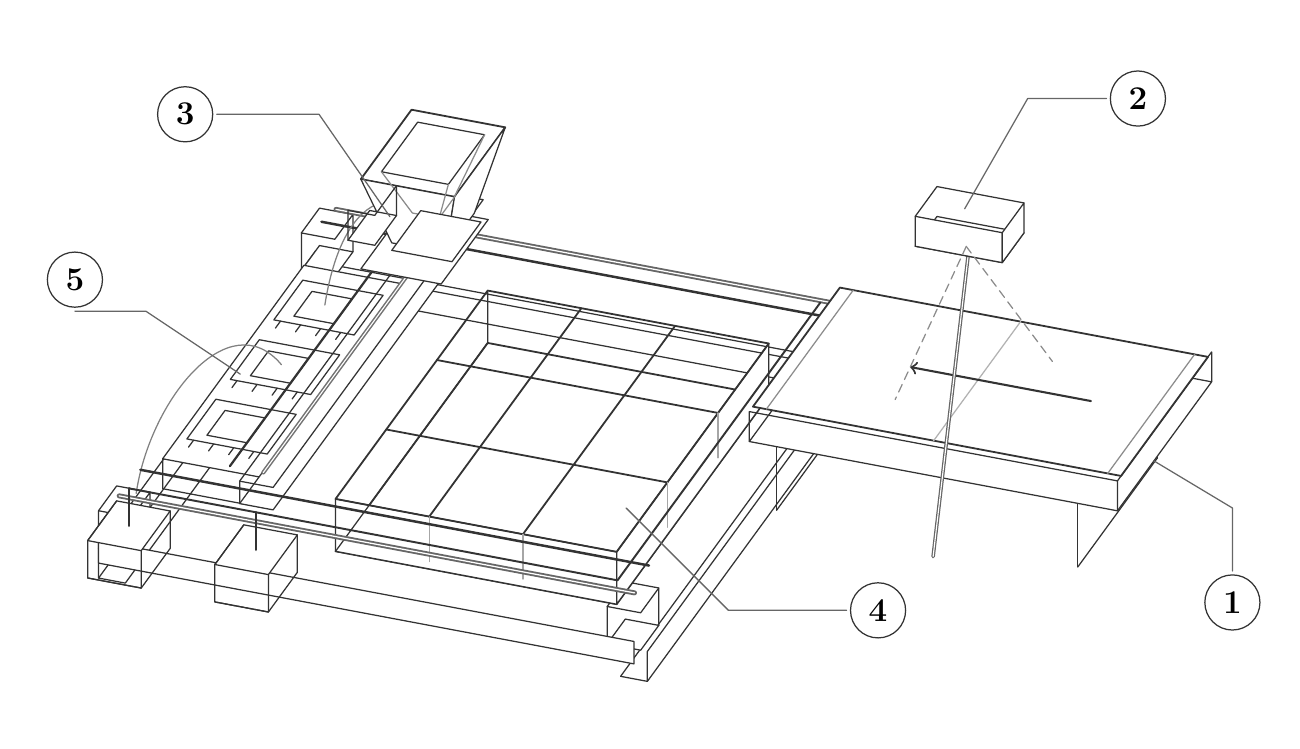
\begin{tikzpicture}[x=1mm,y=1mm,line cap=round,line join=round,
  line width=.45pt,draw=black!80]
\path[use as bounding box] (0,0) rectangle (158,88);
\begin{scope}[shift={(9,20)},x={(.85mm,-.16mm)},
  y={(.46mm,.63mm)},z={(0mm,.95mm)}]
  % Frame and corner supports, far edges first.
  \draw[fill=white] (0,58,-2)--(80,58,-2)--(80,62,-2)--(0,62,-2)--cycle;
  \draw (0,58,-2)--(0,58,2)--(80,58,2)--(80,58,-2);
  \draw[fill=white] (78,0,-2)--(82,0,-2)--(82,60,-2)--(78,60,-2)--cycle;
  \draw (82,0,-2)--(82,0,2)--(82,60,2)--(82,60,-2);
  \draw[fill=white] (0,0,-2)--(4,0,-2)--(4,60,-2)--(0,60,-2)--cycle;
  \draw (0,0,-2)--(0,0,2)--(0,60,2)--(0,60,-2);
  \foreach \frameX in {0,76}{
    \foreach \frameY in {0,56}{
      \draw[fill=white] (\frameX,\frameY,2)--++(5,0,0)--++(0,5,0)--++(-5,0,0)--cycle;
      \draw (\frameX,\frameY,2)--++(0,0,5)--++(5,0,0)--++(0,5,0)--++(0,0,-5);
      \draw (\frameX,\frameY,7)--++(0,5,0)--++(5,0,0);
    }
  }
  % Nine-cell tray with a visible open top and low outside walls.
  \draw[fill=white,line width=.65pt]
    (30,10,0)--(72,10,0)--(72,52,0)--(30,52,0)--cycle;
  \draw[fill=white] (30,10,0)--(72,10,0)--(72,10,7)--(30,10,7)--cycle;
  \draw[fill=white] (72,10,0)--(72,52,0)--(72,52,7)--(72,10,7)--cycle;
  \draw[line width=.65pt] (30,10,7)--(72,10,7)--(72,52,7)--(30,52,7)--cycle;
  \draw (30,10,0)--(30,52,0)--(30,52,7);
  \foreach \cellX in {44,58}{
    \draw[line width=.65pt] (\cellX,10,7)--(\cellX,52,7);
    \draw[black!35] (\cellX,10,7)--(\cellX,10,1);
  }
  \foreach \cellY in {24,38}{
    \draw[line width=.65pt] (30,\cellY,7)--(72,\cellY,7);
    \draw[black!35] (72,\cellY,7)--(72,\cellY,1);
  }
  % Far guide rod and its adjacent belt.
  \draw[line width=1.8pt,black!60] (3,60,8)--(79,60,8);
  \draw[line width=.45pt,white] (3,60,8)--(79,60,8);
  \draw[line width=.9pt] (3,56,9)--(79,56,9);
  % Electronics platform: power module and two driver boards.
  \draw[fill=white] (2,14,5)--(18,14,5)--(18,53,5)--(2,53,5)--cycle;
  \draw (2,14,5)--(2,14,1)--(18,14,1)--(18,53,1)--(18,53,5);
  \foreach \boardY in {17,29,41}{
    \draw[fill=white] (4,\boardY,6)--++(12,0,0)--++(0,8,0)--++(-12,0,0)--cycle;
    \draw (7,\boardY,7)--++(6,0,0)--++(0,5,0)--++(-6,0,0)--cycle;
    \foreach \pinX in {5,8,11,14}{
      \draw (\pinX,\boardY,6)--++(0,-1.4,0);
    }
  }
  % Simplified cable bundle retained as a few uncluttered paths.
  \draw[black!50] (10,44,7) .. controls (6,57,15) and (16,58,15) .. (23,49,14);
  \draw[black!50] (10,32,7) .. controls (0,36,11) and (-1,16,11) .. (4,3,8);
  % Moving bridge spans the storage field.
  \draw[fill=white] (20,2,10)--(25,2,10)--(25,60,10)--(20,60,10)--cycle;
  \draw (20,2,10)--(20,2,13)--(20,60,13)--(20,60,10);
  \draw (20,2,13)--(25,2,13)--(25,60,13)--(20,60,13);
  \draw[line width=1.5pt,black!55] (23,3,14)--(23,59,14);
  \draw[white,line width=.4pt] (23,3,14)--(23,59,14);
  \draw[line width=.8pt] (18,3,14)--(18,58,14);
  % Head carriage and tapered open receiving hopper.
  \draw[fill=white] (17,41,15)--(29,41,15)--(29,54,15)--(17,54,15)--cycle;
  \draw[fill=white,line width=.65pt]
    (17,41,27)--(31,41,27)--(31,55,27)--(17,55,27)--cycle;
  \draw[fill=white] (17,41,27)--(20,44,17)--(28,44,17)--(31,41,27)--cycle;
  \draw[fill=white] (31,41,27)--(28,44,17)--(28,52,17)--(31,55,27)--cycle;
  \draw (19,43,27)--(29,43,27)--(29,53,27)--(19,53,27)--cycle;
  \draw[black!45] (19,43,27)--(22,46,20)--(26,46,20)--(29,43,27);
  \draw[black!45] (26,46,20)--(26,50,20)--(29,53,27);
  \draw[fill=white] (20,44,16)--(29,44,16)--(29,52,16)--(20,52,16)--cycle;
  % Small servo body on the side of the head.
  \draw[fill=white] (14,43,17)--(18,43,17)--(18,49,17)--(14,49,17)--cycle;
  \draw (14,43,17)--(14,43,21)--(18,43,21)--(18,49,21)--(18,49,17);
  % Conveyor, on a separate stand to the right of the frame.
  \foreach \standX in {84,129}{
    \draw (\standX,32,0)--(\standX,32,12);
    \draw (\standX,54,0)--(\standX,54,12);
    \draw (\standX,32,0)--(\standX,54,0);
  }
  \draw[fill=white] (81,30,10)--(136,30,10)--(136,56,10)--(81,56,10)--cycle;
  \draw (81,30,10)--(81,30,14)--(136,30,14)--(136,30,10);
  \draw (136,30,14)--(136,56,14)--(136,56,10);
  \draw[fill=white,line width=.65pt] (81,31,14)--(136,31,14)--(136,55,14)--(81,55,14)--cycle;
  \draw[black!45] (83,31,14)--(83,55,14);
  \draw[black!45] (134,31,14)--(134,55,14);
  \draw[black!30] (108,31,14)--(108,55,14);
  % Arrow denotes the physical direction of feeding.
  \draw[line width=.75pt,->] (125,43,14.2)--(98,43,14.2);
  % Camera support and camera above the viewing zone.
  \draw[line width=1.3pt,black!60] (109,29,0)--(109,39,35);
  \draw[line width=.4pt,white] (109,29,0)--(109,39,35);
  \draw[fill=white] (102,37,35)--(115,37,35)--(115,43,35)--(102,43,35)--cycle;
  \draw[fill=white] (102,37,35)--(102,37,39)--(115,37,39)--(115,37,35)--cycle;
  \draw[fill=white] (115,37,35)--(115,37,39)--(115,43,39)--(115,43,35)--cycle;
  \draw (102,37,39)--(102,43,39)--(115,43,39);
  \draw[black!45,densely dashed] (108,40,34)--(99,37,14);
  \draw[black!45,densely dashed] (108,40,34)--(116,49,14);
  % Front frame rail, belt and motor housings.
  \draw[fill=white] (0,0,0)--(80,0,0)--(80,0,3)--(0,0,3)--cycle;
  \draw[line width=1.8pt,black!60] (2,2,8)--(79,2,8);
  \draw[line width=.45pt,white] (2,2,8)--(79,2,8);
  \draw[line width=.9pt] (3,6,9)--(79,6,9);
  \foreach \motorX in {0,19}{
    \draw[fill=white] (\motorX,-3,5)--++(8,0,0)--++(0,8,0)--++(-8,0,0)--cycle;
    \draw (\motorX,-3,5)--++(0,0,-5)--++(8,0,0)--++(0,8,0)--++(0,0,5);
    \draw (\motorX,-3,0)--++(8,0,0)--++(0,0,5);
    \draw (\motorX,-3,5)--++(0,8,0);
  }
  \draw[line width=1pt] (4,1,5)--(4,1,10);
  \draw[line width=1pt] (23,1,5)--(23,1,10);
  \draw[line width=.7pt] (4,1,10)--(77,1,10)--(77,57,10);
\end{scope}
% The leaders sit outside the geometry and are independent of its projection.
\draw[black!60] (143,33)--(153,27)--(153,19);
\draw[black!60] (119,65)--(127,79)--(137,79);
\draw[black!60] (46,64)--(37,77)--(24,77);
\draw[black!60] (76,27)--(89,14)--(104,14);
\draw[black!60] (27,44)--(15,52)--(6,52);
\foreach \labelX/\labelY/\labelNumber in {153/15/1,141/79/2,20/77/3,108/14/4,6/56/5}{
  \node[draw=black!80,fill=white,circle,inner sep=0pt,minimum size=7mm,
    font=\bfseries\fontsize{12bp}{12bp}\selectfont]
    at (\labelX,\labelY) {\labelNumber};
}
\end{tikzpicture}
